\section{Dataset}

\subsection{CelebA}

CelebA is a large-scale face attributes dataset with more than 200K celebrity images, each with 40 attribute annotations. The images in this dataset cover large pose variations and background clutter. CelebA has large diversities, large quantities, and rich annotations, including \textbf{5,000 celebrity identities}, \textbf{202,599 face images}, and \textbf{40 binary attributes} annotations per image. The dataset can be employed as the training and test sets for the following computer vision tasks: face attribute recognition, face detection, landmark (or facial part) localization, and face editing/synthesis.

% insert the image of the dataset
\begin{figure}[h]
\centering
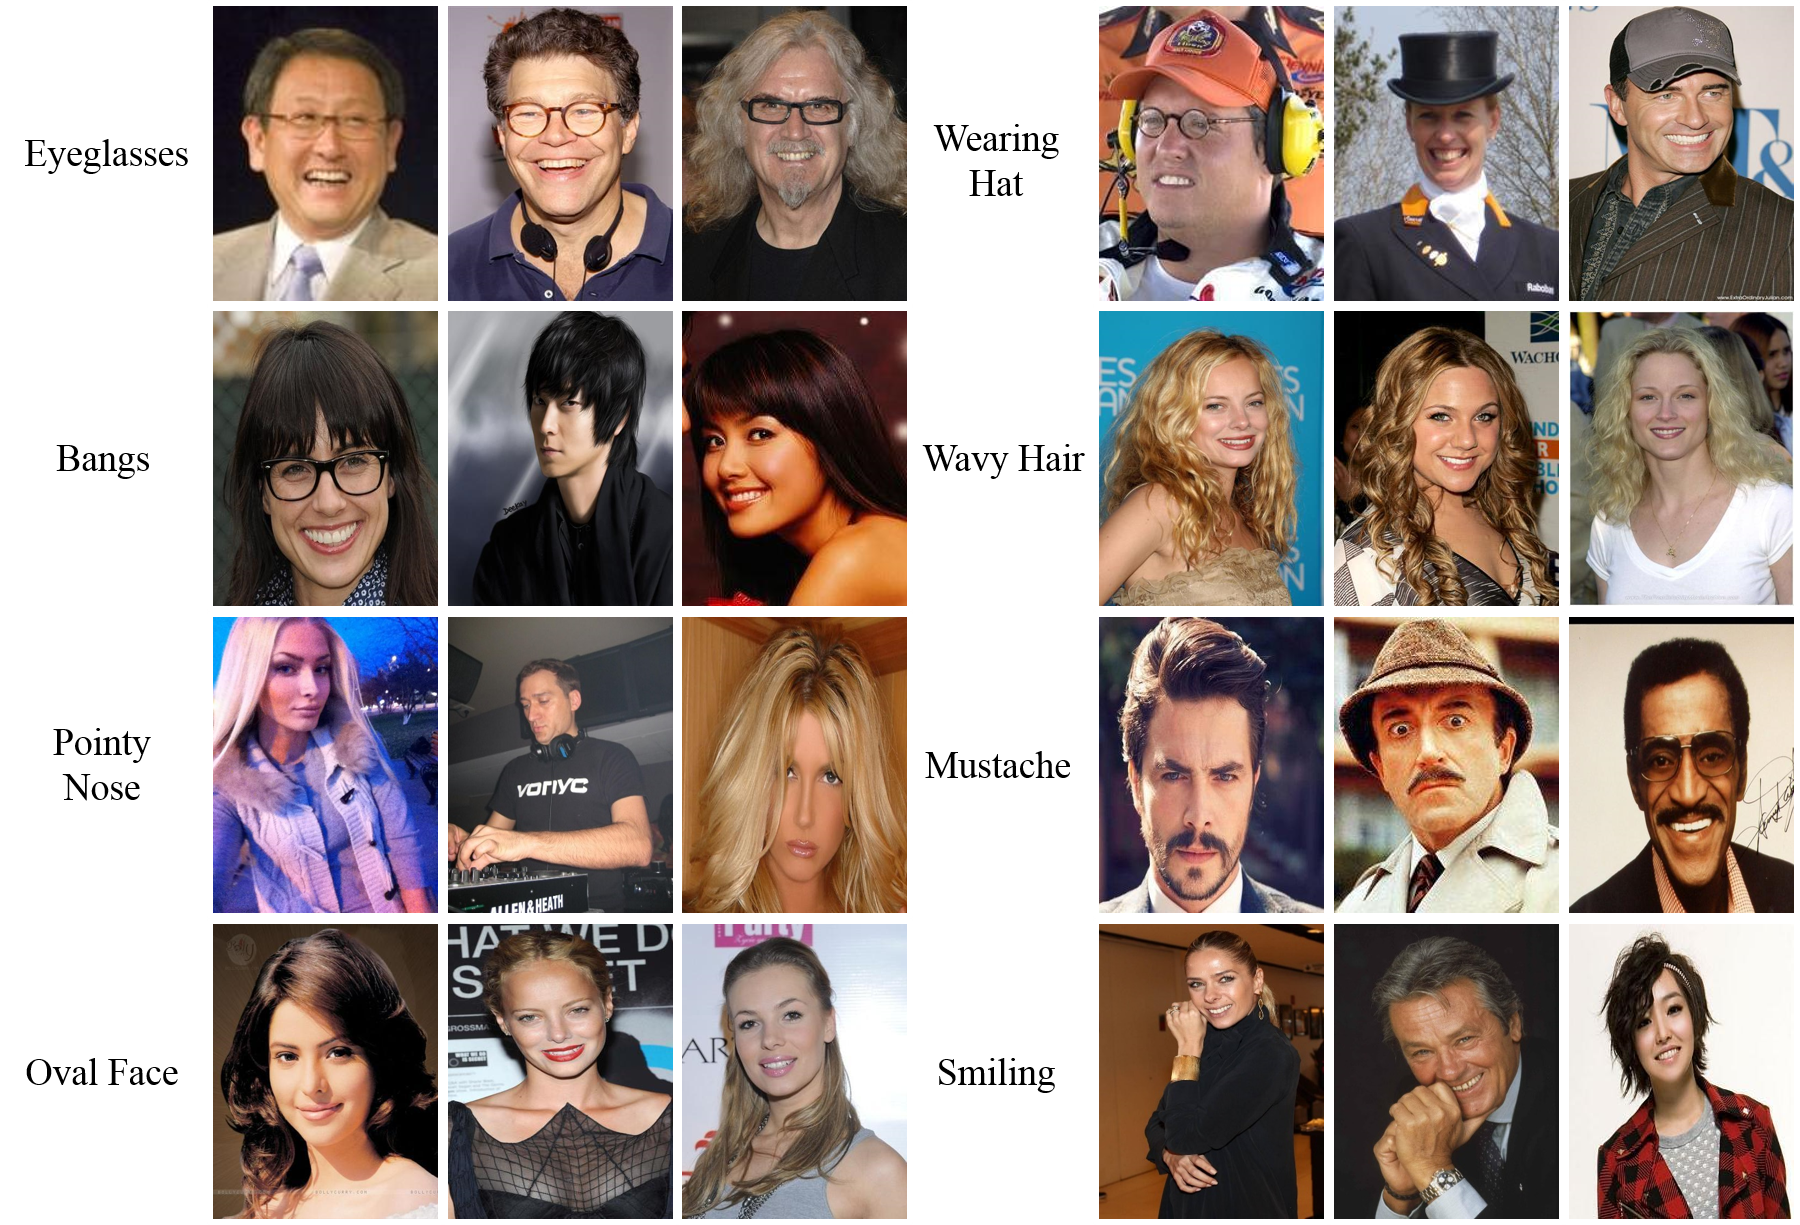
\includegraphics[width=0.5\textwidth]{CelebA}
\caption{CelebA dataset}
\label{fig:CelebA}
\end{figure}

CelebA is utilised as the face recognition model's dataset set in this project. The training set has 4429 photos while the test set has 1267 images.

\subsection{Private Dataset}

The private dataset consists of photos collected by team members. The photos were taken in SITE and feature various facial expressions.

This dataset is utilized to perform adversarial attacking on the face recognition model. The training set has 121 photos while the test set has 15 images.

